\def\QRCODE{TB_IPR_TUT.IMG.pixel_topological_description_matlabqrcode.png}
\def\QRPAGE{http://www.iptutorials.science/tree/master/TB_IPR/TUT.IMG.pixel_topological_description/matlab}
\mcorrectionsection{Matlab correction}

%\begin{mcomment}
%\begin{mremark}
%Please notice that when using boolean arrays in matlab, the notations $1-X$ and $\sim X$ are equivalent. When using uint8 arrays, verify that the values range into [0;1].
%\end{mremark}
%\end{mcomment}

\subsection{Toplogical description}
The connectivity numbers are computed in the following way:
\begin{matlab}
function [T8,T8c,TT8]=nc(A)
% A : block 3x3, binary

% complementary set of A
invA=1-A;

% neighborhoods
V8=ones(3,3);
V8_star=[1 1 1;1 0 1;1 1 1];
V4=[0 1 0;1 1 1;0 1 0];

% intersection is done by the min operation
X1=min(V8_star,A);
TT8=sum(X1(:));
[~, T8] = bwlabeln(X1,8);

% The C-ajd-4 might introduce some problems if a pixel is not 4-connected
% to the central pixel
X2=min(V8,invA);
Y=min(X2,V4);
X=imreconstruct(Y,X2,4);
[~, T8c]=bwlabeln(X,4);

\end{matlab}
\noindent They are here applied on the original 'test' image at the specific point with coordinates $(2,5)$:
\begin{matlab}
% reading image
A=imread('test.bmp');
A=double(A(:,:,1));
A=A/255;
figure;
x=[2 5];
X=A(x(1)-1:x(1)+1,x(2)-1:x(2)+1);
subplot(1,2,1);viewImage(A);title('original image');
subplot(1,2,2);viewImage(X);title('3x3 window centered on the point (2,5)');
% connectivity numbers
[nc1,nc2,nc3]=nc(X)
\end{matlab}

The current 3x3 window is represented in Fig.\ref{fig:topological_description:matlab:3x3window}.

\begin{figure}[htbp]
 \centering
 %\subfloat[Original image.]{
 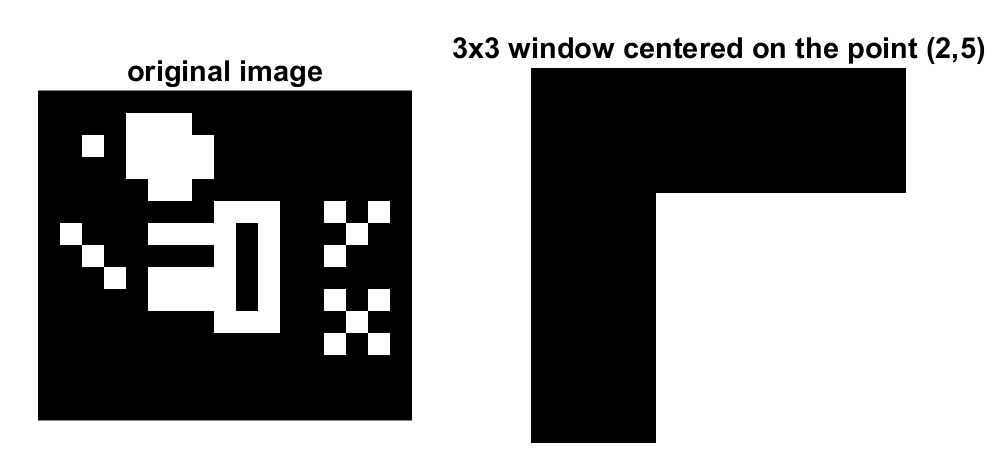
\includegraphics[width=8cm]{3x3window.png}
 %}\hspace*{1cm}
 \caption{Representation of the current 3x3 window.}
 \label{fig:topological_description:matlab:3x3window}
\end{figure}

giving the following connectivity numbers:

\begin{mwindow}
nc1 = 1
nc2 = 1
nc3 = 3 
\end{mwindow}


\subsection{Topological classification of binary points}
The following function gives the classification of the current point according to the 3 connectivity numbers. Note that the topological description of a point is given by a value between 1 and 7.
\begin{matlab}
function y=nc_type(n);
[a,b,c]=nc(n);
if (a==0) y=1;end % isolated point
if ((a==1) && (b==1) && (c>1)) y=5;end  % border point
if (b==0) y=7;end % interior point
if ((a==1) && (b==1) && (c==1)) y=6;end % end point
if (a==2) y=2;end % 2-junction point
if (a==3) y=3;end % 3-junction point
if (a==4) y=4;end % 4-junction point
\end{matlab} 
\noindent Consequently, each point of a binary image can now be topologically classified:
\begin{matlab}
% for the whole image
[m,n]=size(A);
B=zeros(m,n);
for i=2:m-1
    for j=2:n-1
        if A(i,j)> 0
            X=A(i-1:i+1,j-1:j+1);
            B(i,j)=nc_type(X);
        end
    end
end
disp('Point classification :');
disp('1 : isolated points');
disp('2 : 2-junction points');
disp('3 : 3-junction points');
disp('4 : 4-junction points');
disp('5 : border points');
disp('6 : end points');
disp('7 : interior points');

subplot(3,3,1);viewImage(A);title('original image');
subplot(3,3,2);viewImage(B);title('point classification');
subplot(3,3,3);viewImage(B==5);title('border points');
subplot(3,3,4);viewImage(B==7);title('interior points');
subplot(3,3,5);viewImage(B==1);title('isolated points');
subplot(3,3,6);viewImage(B==6);title('end points');
subplot(3,3,7);viewImage(B==2);title('2-junction points');
subplot(3,3,8);viewImage(B==3);title('3-junction points');
subplot(3,3,9);viewImage(B==4);title('4-junction points');
\end{matlab} 
\noindent with the following result:
\begin{figure}[htbp]
 \centering
 %\subfloat[Original image.]{
 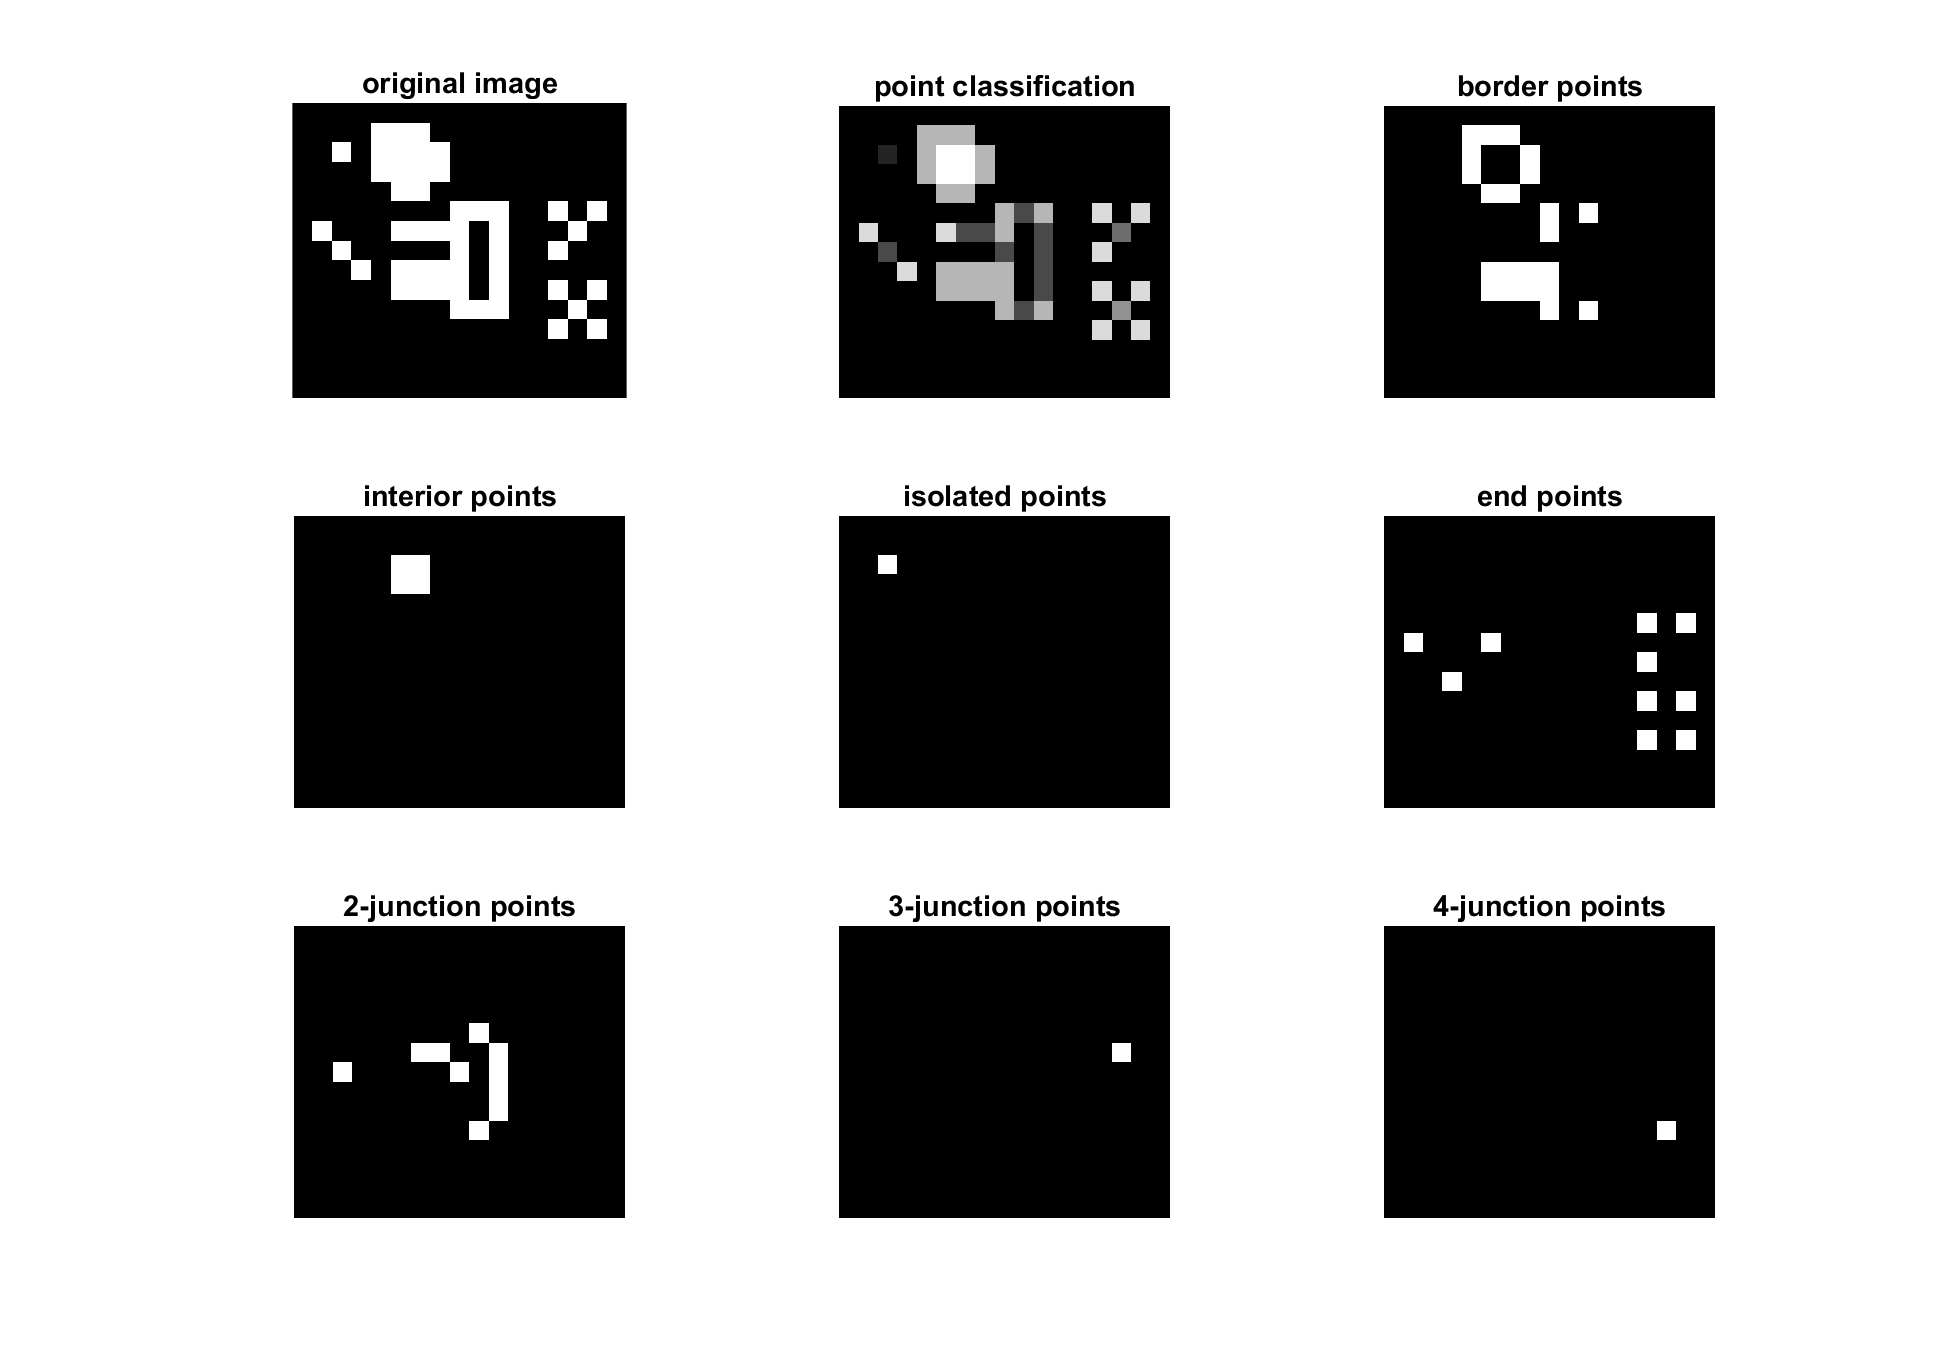
\includegraphics[width=\textwidth]{imageClassification.png}\label{fig:topological_description:matlab:imageClassification}
 %}\hspace*{1cm}
 \caption{Topological classification of the image points.}
\end{figure}

\noindent Note that the following function \texttt{viewImage} has been used to display the different images of this tutorial:
\begin{matlab}
function viewImage(A)
B=double(A);
mmax=max(max(B));
mmin=min(min(B));
if (mmax == mmin) B=0;
else B=uint8(255*(B-min(min(B)))/(max(max(B))-min(min(B))));
end
colormap gray;axis image;
imshow(B);
\end{matlab}
